% Set page size and margins
\usepackage[
  a4paper,
  top=2cm,
  bottom=3cm,
  left=2cm,
  right=2cm,
  marginparwidth=1.75cm,
  footskip=2.05cm,
]{geometry}

% Useful packages
\usepackage[export]{adjustbox}
\usepackage{amsmath}
\usepackage{array}
\usepackage{caption}
\usepackage[strict]{changepage}
\usepackage{enumitem}
\usepackage{etoolbox}
\usepackage{float}
\usepackage{fullwidth}
\usepackage{graphicx, trimclip}
\usepackage[colorlinks=true, allcolors=blue]{hyperref}
\usepackage{hyperref}
\usepackage[noautomatic, nonewpage]{imakeidx}
\usepackage{multicol}
\usepackage[super]{nth}
\usepackage{outlines}
\usepackage{paracol}
\usepackage[section]{placeins}
\usepackage{setspace}
\usepackage{stfloats}
\usepackage{subcaption}
\usepackage[usetransparent=false]{svg}
\usepackage{tabularx}
\usepackage[subfigure]{tocloft}
\usepackage{tikz}
\usepackage{titlesec}
\usepackage{verbatim}
\usepackage{varwidth}
\usepackage{wrapfig}
\usepackage[most]{tcolorbox}
\usepackage{catchfile}
\usepackage{xstring}
\usepackage{soul}
\usepackage{xifthen}
\usepackage[para, symbol, perpage]{footmisc}
\newtcolorbox{scaledfigure}[1][]{height fill, space to=\myspace,#1}
\hypersetup{
  colorlinks=true,
  linkcolor=goldenbrown,
  filecolor=magenta,
  urlcolor=cyan,
  pdftitle={Heroes of Might \& Magic III Fan-Made Mission Book},
  pdfpagemode=UseNone,
}
% Set the default spacing between paragraphs. Remove indentation.
\usepackage[skip=6pt, indent=0pt]{parskip}
\setstretch{1}

% Get version from env
% \getenv{variable_name} just prints the value
% \getenv[\macro]{variable_name} stores the value in \macro for reusability
\newcommand{\getenv}[2][]{%
  \CatchFileEdef{\value}{"|echo \$#2"}{\endlinechar=-1}%
  \if\relax\detokenize{#1}\relax\value\else\let#1\value\fi}

% Add dots to the table of contents
\renewcommand{\cftsecleader}{\cftdotfill{\cftsecdotsep}}
\renewcommand\cftsecdotsep{\cftdot}
\renewcommand\cftsubsecdotsep{\cftdot}

\captionsetup[figure]{labelformat=empty}
\captionsetup[subfigure]{labelformat=empty, singlelinecheck=off, justification=centering}
\usetikzlibrary{shadows, shadows.blur, calc, backgrounds}

\setlength{\columnsep}{1cm}
\newtoggle{printable}
\newtoggle{noartbackground}
\newtoggle{githubbuild}

% Variables
\def\_assets{assets}

\def\art{\_assets/art}
\def\cards{\_assets/cards}
\def\examples{\_assets/examples}
\def\images{\_assets/images}
\def\layout{\_assets/layout}
\def\map_locations{\_assets/map-locations}
\def\skills{\_assets/skills}
\def\spells{\_assets/spells}
\def\svgs{\_assets/glyphs}
\def\notes_svgs{\svgs/for-notes}
\def\tables{\_assets/tables}
\def\qr{\_assets/qr-codes}

\def\repourl{https://github.com/Heegu-sama/Homm3BG}
\def\bggthreadurl{https://boardgamegeek.com/thread/3235221/rule-book-rewrite-project}

\newcommand{\svg}[2][]{%
  \ifthenelse{\equal{#1}{}}%
  {\includesvg[height=10px]{\svgs/\detokenize{#2}.svg}}%
  {\includesvg[height=#1px]{\svgs/\detokenize{#2}.svg}}%
}%

\renewcommand{\labelitemi}{
\includegraphics[width=0.7em, valign=c]{\layout/listdot.png}}

% Colors
\definecolor{amber}{rgb}{1.0, 0.49, 0.0}
\definecolor{antiquewhite}{rgb}{0.98, 0.92, 0.84}
\definecolor{arylideyellow}{rgb}{0.96, 0.89, 0.58}
\definecolor{cadmiumgreen}{rgb}{0.0, 0.42, 0.24}
\definecolor{darkcandyapplered}{rgb}{0.64, 0.0, 0.0}
\definecolor{goldenbrown}{rgb}{0.6, 0.4, 0.08}

% Command to frame images
\newcommand\framedimage[2][]{%
  \begin{tikzpicture}
    \draw (0, 0) node[inner sep=0] {\makebox[#1][c]{\includegraphics[width=#1]{#2}}};
    \draw [bordermidyellow, thick] ([xshift=+1pt, yshift=-1pt] current bounding box.north west) rectangle ([xshift=-1pt, yshift=1pt] current bounding box.south east);
    \draw [borderoutyellow, thick] (current bounding box.north west) rectangle (current bounding box.south east);
    \draw [borderinyellow, thick] ([xshift=+3pt, yshift=-3pt] current bounding box.north west) rectangle ([xshift=-3pt, yshift=3pt] current bounding box.south east);
  \end{tikzpicture}}
% End of drop frame definition

\titleformat{\section}
{\huge}
{\filright
\footnotesize
\enspace SECTION \thesection\enspace}
{8pt}
{\Huge\bfseries\filcenter\uppercase}
%Create section heading with graphics. Argument one is heading name, argument two is picture to use on the left.
\providecommand{\sectionheadertext}[1]{
  \fontfamily{ptm}\selectfont{
    \color{antiquewhite} \section*{\MakeUppercase{#1}}
  }
}
\newcommand{\addsection}[2]{
  \vspace*{-5em}
  \hspace*{-1em}
  \makebox[0pt][l]{
  \raisebox{-\totalheight}[0pt][7pt]{
    \begin{tikzpicture}
      \draw (0, 0) node[inner sep=0] {
\includegraphics[width=\linewidth, height=0.2\linewidth]{\layout/section_heading.jpg}};
      \draw (-6.2, 0) node {\includegraphics[width=0.125\textwidth]{#2}};
    \end{tikzpicture}
    }
  }
  \begin{fullwidth}[leftmargin=0.16\textwidth, outermargin=0.16\textwidth, innermargin=0.16\textwidth]
    \begin{center}
      \vspace*{\lang_header_adjustment}
      \sectionheadertext{#1}
      \cleardoublepage\phantomsection\addcontentsline{toc}{section}{\protect\numberline{}#1}
    \end{center}
  \end{fullwidth}
  \vspace{1.75em}
}
%End of create section heading.

% Four mandatory params
% - lines of campaign name (1-2 according to the name length)
% - campaign name
% - scenario name
% - icon
%
% TODO: possibly replace the whole \addsection with this
\newcommand{\addscenariosection}[4]{
  \sodef\sotitle{}{0.2em}{0.6em}{1.2em}
  \def\oneliner{\equal{#1}{1}}

  \vspace*{-5em}
  \hspace*{-1.3em}
  \makebox[0pt][l]{
  \raisebox{-\totalheight}[0pt][7pt]{
    \ifthenelse{\oneliner}{\def\yscale{1}}{\def\yscale{1.3}}
    \begin{tikzpicture}
      \draw (0, 0) node[inner sep=0, yscale=\yscale] {
\includegraphics[width=\linewidth, height=0.2\linewidth]{\layout/section_heading.jpg}};
      \draw (-6.2, 0) node {\includegraphics[width=0.125\textwidth]{#4}};
    \end{tikzpicture}
    }
  }
  \begin{fullwidth}[leftmargin=0.16\textwidth]
    \begin{center}
      \vspace{-22pt}
      \sectionheadertext{\small{\sotitle{#2}}}
      \vspace{-12pt}
      \sectionheadertext{#3}
      \ifthenelse{\oneliner}{}{\vspace{14pt}}
      \cleardoublepage\phantomsection\addcontentsline{toc}{section}{\protect\numberline{}#3}
    \end{center}
  \end{fullwidth}
  \ifthenelse{\oneliner}{\vspace{1.75em}}{\vspace{2.75em}}
}

% Apply language-specific subsection spacings if defined
\ifdefined\subsectionspacing
  \subsectionspacing{}
\fi

\newcommand\picdims[4][]{%
  \setbox0=\hbox{\includegraphics[#1]{#4}}%
  \clipbox{.5\dimexpr\wd0-#2\relax{} %
    .5\dimexpr\ht0-#3\relax{} %
    .5\dimexpr\wd0-#2\relax{} %
    .5\dimexpr\ht0-#3\relax}{\includegraphics[#1]{#4}}}

\tikzset{
  thick/.style=      {line width=1.3pt},
  very thick/.style= {line width=1.7pt},
  ultra thick/.style={line width=2.2pt}
}

\definecolor{borderoutyellow}{HTML}{DBCA86}
\definecolor{borderinyellow}{HTML}{B09E69}
\definecolor{bordermidyellow}{HTML}{6f6749}
% Create note box
\providecommand{\notefont}[0]{\fontfamily{ptm}\selectfont}
\newcommand{\note}[2]{
  \begin{tikzpicture}
    \draw (0, 0) node[inner sep=0] {\makebox[\linewidth][c]{\picdims[width=\linewidth]{\linewidth}{#1\baselineskip}{\layout/table-background.jpg}}};
    \draw [borderoutyellow, very thick] (current bounding box.north west) rectangle (current bounding box.south east);
    \draw [borderinyellow, thick] ([xshift=+2.8pt, yshift=-2.8pt] current bounding box.north west) rectangle ([xshift=-2.8pt, yshift=2.8pt] current bounding box.south east);
    \node at (current bounding box.center) {
      \begin{varwidth}{0.85\linewidth}
      \notefont{
        \color{arylideyellow}
        \hypersetup{linkcolor=amber}
        #2
        \hypersetup{linkcolor=goldenbrown}
      }
      \end{varwidth}
    };
    \begin{pgfonlayer}{background}
      \begin{scope}[blend mode=multiply]
        \draw [shade, blur shadow={shadow opacity=15}] (current bounding box.north west) rectangle (current bounding box.south east);
      \end{scope}
    \end{pgfonlayer}
  \end{tikzpicture}
}

% Create Heroes-styled framed canvas for a table. Accepts three arguments:
% 1) [Optional] Drop shadow description. Use [] as the first arg to delete it.
% 2) Height specified in verses (lines of text)
% 3) Table contents like title and tabularx environment
\newcommand{\hommtable}[3][shade, blur shadow={shadow opacity=15}]{
  \begin{tikzpicture}
    \draw (0, 0) node[inner sep=0] {\makebox[\linewidth][c]{\picdims[width=\linewidth]{\linewidth}{#2\baselineskip}{\layout/table-background.jpg}}};
    \draw [bordermidyellow, thick] ([xshift=+1pt, yshift=-1pt] current bounding box.north west) rectangle ([xshift=-1pt, yshift=1pt] current bounding box.south east);
    \draw [borderoutyellow, thick] (current bounding box.north west) rectangle (current bounding box.south east);
    \draw [borderinyellow, thick] ([xshift=+3pt, yshift=-3pt] current bounding box.north west) rectangle ([xshift=-3pt, yshift=3pt] current bounding box.south east);
    \node at (current bounding box.center) {
      \begin{varwidth}{0.95\linewidth}
      \notefont{
        \bgroup
        \color{arylideyellow}
        \hypersetup{linkcolor=amber}
        \setlength{\tabcolsep}{0.3em}
        #3
        \egroup
      }
      \end{varwidth}
    };
    \begin{pgfonlayer}{background}
      \begin{scope}[blend mode=multiply]
        \draw [#1] (current bounding box.north west) rectangle (current bounding box.south east);
      \end{scope}
    \end{pgfonlayer}
  \end{tikzpicture}
}
% End of Heroes-styled canvas definition.

\definecolor{darkcellborder}{HTML}{634831}
\definecolor{darkcellbg}{HTML}{20160C}

\newcommand{\darkcell}[2][0.9]{
  \begin{tikzpicture}
    \filldraw[line width=1.0pt, fill=darkcellbg, fill opacity=0.5, draw=darkcellborder] (0, 0) rectangle (\linewidth, #1);
    \node[text width=\linewidth, align=center] at (current bounding box.center) {\textbf{#2}};
  \end{tikzpicture}
}

\definecolor{lightcellborder}{HTML}{77543e}
\definecolor{lightcellbg}{HTML}{20160C}

\newcommand{\lightcell}[2][0.9]{
  \begin{tikzpicture}
    \filldraw[line width=1.0pt, fill=lightcellbg, fill opacity=0.25, draw=lightcellborder] (0, 0) rectangle (\linewidth, #1);
    \node[text width=\linewidth, align=center] at (current bounding box.center) {\color{white}#2};
  \end{tikzpicture}
}

% Commands to be used for automation generating printable version
\newcommand{\pagetarget}[2]{\label{#1}\hypertarget{#1}{#2}}
\newcommand{\pagelink}[2]{\hyperlink{#1}{#2}\iftoggle{printable}{ \textmd{(\pageshorthand\,\pageref{#1})}}{}}

% Command for overlay circled text
\definecolor{goblin}{HTML}{3b7c33}
\newcommand\encircle[1]{%
  \tikz[baseline=(X.base)]
  \node (X) [draw=white, shape=circle, inner sep=0, fill=goblin, text=white, blur shadow={shadow blur steps=5}] {\strut \textbf{#1}};%
}

% Background
\AddToHook{shipout/background}{%
  \iftoggle{noartbackground}{}{
    \put (0in,-\paperheight){\includegraphics[width=\paperwidth,height=\paperheight]{\layout/tausta.png}}
  }
  \iftoggle{printable}{
    \ifodd\value{page}
      \put (0in,-\paperheight){\includegraphics[width=\paperwidth]{\layout/bottom-odd.png}}
    \else
      \put (0in,-\paperheight){\includegraphics[width=\paperwidth,height=0.05\paperheight]{\layout/bottom-even.png}}
    \fi
  }{\put (0in,-\paperheight){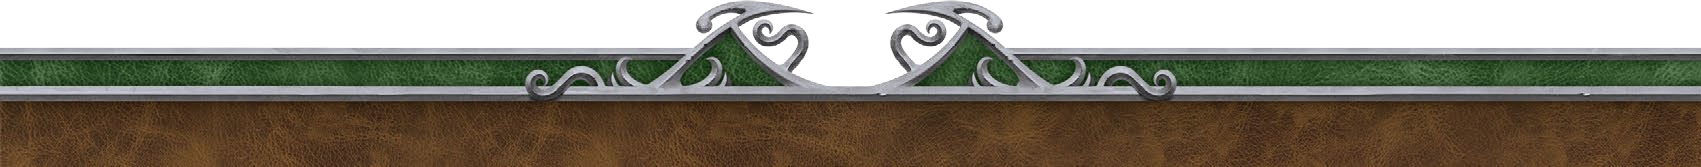
\includegraphics[width=\paperwidth,height=0.05\paperheight]{\layout/bottom.png}}}
}

\makeindex[columns=3, title=,]

\begin{document}

% !TeX spellcheck = en_US
\thispagestyle{empty}
\begin{tikzpicture}[remember picture, overlay, inner sep=10pt]
  \iftoggle{noartbackground}{}{
    \node(cover)[anchor=center] at (current page.center) {
      \includegraphics[height=\paperheight, keepaspectratio]{\layout/cover.jpg}
    };
  }
  \node(title)[minimum width = \paperwidth, anchor=center, yshift=\dimexpr-10em\relax] at (current page.north) {
    \includegraphics[width=0.6\paperwidth]{\layout/cover_title.png}
  };
  \node(subtitle)[anchor=center, yshift=12em] at (current page.south) {
    
\includegraphics[width=0.6\paperwidth]{\layout/cover_subtitle.png}
  };
\end{tikzpicture}

% Render phantom SVGs before their use in tabular env
\phantom{
  \includesvg[height=0.1px]{\svgs/bronze.svg}
  \includesvg[height=0.1px]{\svgs/bronze.svg}
  \includesvg[height=0.1px]{\svgs/silver.svg}
  \includesvg[height=0.1px]{\svgs/golden.svg}
  \includesvg[height=0.1px]{\svgs/azure.svg}
  \includesvg[height=0.1px]{\svgs/gold.svg}
  \includesvg[height=0.1px]{\svgs/building_materials.svg}
  \includesvg[height=0.1px]{\svgs/valuables.svg}
  \includesvg[height=0.1px]{\svgs/attack-yellow.svg}
  \includesvg[height=0.1px]{\svgs/defense-yellow.svg}
  \includesvg[height=0.1px]{\svgs/damage-yellow.svg}
}


\iftoggle{printable}{
  \newgeometry{
    twoside,
    top=2cm,
    bottom=3cm,
    left=2.5cm,
    right=1.5cm,
    marginparwidth=1.75cm,
    footskip=2.05cm,
  }
}{}

\author{By The Community}
\maketitle

\begin{center}
  \iftoggle{githubbuild}{
    \getenv[\githubsha]{GITHUB_SHA}
    \versionwarning{} \href{\repourl}{\StrLeft{\githubsha}{7}}.
  }{
    \versionlabel{} \input{.version}
  }

  \bigbreak

  \intro{}

  \bigbreak\authorsquote
\end{center}

\iftoggle{printable}{
  \bigbreak

  \begin{multicols}{2}
  \centering
  
\includegraphics[width=0.8\linewidth]{\qr/github.png}\\
  \qrgithub

  \columnbreak

  \includegraphics[width=0.8\linewidth]{\qr/bgg.png}\\
  \qrbgg
  \end{multicols}
}{}

\begin{tikzpicture}[remember picture, overlay]
  \node(cover)[anchor=center, yshift=12em] at (current page.south) {
    \includegraphics[width=1.01\paperwidth, keepaspectratio]{\art/castle_bottom.png}
    \thispagestyle{empty}
  };
\end{tikzpicture}

\clearpage

\begin{multicols*}{2}
\tableofcontents
\vspace*{\fill}
\columnbreak
\vspace*{\fill}
\includegraphics[width=\linewidth]{\art/mummy.jpg}
\end{multicols*}

\clearpage

% !TeX spellcheck = en_US
\addscenariosection{1}{Cooperative scenario}{Sentinels}{\images/sentinel.png}

\begin{multicols*}{2}

\textbf{Author:} silence70011

\textbf{Source:} \href{https://discord.com/channels/740870068178649108/1233112440322002964/1233112440322002964}{Archon Studio Discord}

\subsection*{\MakeUppercase{Scenario length}}

This scenario plays out over 12 rounds.

\subsection*{\MakeUppercase{Player setup}}

\textbf{Player count:} 2

\textbf{Starting Resources:} 10 \svg{gold}, 2 \svg{building_materials}, 1 \svg{valuables}

\textbf{Starting Income:} 10 \svg{gold}, 2 \svg{building_materials}, 1 \svg{valuables}

\textbf{Starting Units:} 
    A Pack of \svg{bronze} units with the \textit{lowest} recruitment cost. 
    A Few \svg{bronze} units with the \textit{highest} recruitment cost 

\textbf{Town Buildings:} \svg{bronze} Dwelling, Citadel

\textbf{Map Tile Pool:} Each player takes 1 random Near Map Tile (IV-V) and 1 random Far Map Tile (II-III).

\textbf{Bonus:} Search (2) the Artifact Deck 

\subsection*{\MakeUppercase{Map setup}}

Take the following Map tiles and set them up as shown in the scenario map layout:

\textbf{2 × Starting Map tile (I)}
\begin{itemize}
    \item Starting Tiles of your chosen factions.
    \item Ignore their yellow borders.
\end{itemize}

\textbf{4 × Far Map tile (II-III)}

\textbf{4 × Near Map tile (IV-V)}
\begin{itemize}
    \item All Near Map tiles must have obelisks.
\end{itemize}

\subsection*{\MakeUppercase{Additional rules}}

\begin{itemize}
    \item Players can trade resources when the one of the active player's heroes 
    visits a trading post or stands on a field adjacent to an allied hero.
    \item The hero who defeats an enemy army gains 2 \svg{experience}.
    The winning player throws two Treasure Dice and chooses one.
\end{itemize}

\subsection*{\MakeUppercase{Win/lose conditions}}

\textbf{Win:}
\begin{itemize}
    \item Defeat all invading armies.
\end{itemize}

\textbf{Lose:}
\begin{itemize}
    \item There is an undefeated enemy army left by the end of Round 12.
    \item One of your towns is captured or a main hero is defeated in battle 
    (retreat doesn't count).
\end{itemize}

\subsection*{\MakeUppercase{Timed events}}

\textbf{6$^{th}$ and 9$^{th}$ Round:}
\begin{itemize}
    \item Remove black cubes from windmills, water wheels and mystical gardens.
\end{itemize}

\textbf{6-10$^{th}$ Rounds:}
\begin{itemize}
    \item Spawn an enemy army according to the rules below.
\end{itemize}

\subsection*{\MakeUppercase{The story}}

There is a world beyond this world and it is filled with beasts and monsters, 
barely held captive by a formation of four sacred obelisks.

But the protection of the stones is weakening and a breach is imminent.

When it happens only you and your ally stand between the hordes and total 
devastation of these lands.

\end{multicols*}

\newpage

\subsection*{\MakeUppercase{Enemy spawning and movement}}

\begin{itemize}
    \item Enemy armies spawn on a random obelisk field (use hero miniatures of factions not in play).
    \item Determine which obelisk field by rolling 2 Attack Dice
    \begin{itemize}
        \item First die: --1 west, +1 east, 0 reroll
        \item Second die: --1 north, +1 south, 0 reroll
    \end{itemize}
    \item For more equal distribution, in rounds 7 and 9 the enemy spawns on the opposite side
    than in the round before. Rounds 8 and 10 are all random.
    \item If the tile to spawn an enemy on isn't discovered yet, flip it over and orient as preferred.
    \item If there is a hero on the field where the enemy spawns, a fight is initiated immediately.
    \item Enemy armies move at the end of every turn, starting with the same turn they spawned.
    \item Enemy armies have 3 Movement Points per round.
    \item Enemy armies move as described in the rulebook (p. 33) but instead of capturing they destroy
    everything in their way. Place black cubes on any field they pass and treat them as empty from that point.
    \item If an enemy's movement could go two different ways the players decide which way to go.
\end{itemize}

\subsection*{\MakeUppercase{Combat with enemy armies}}

\begin{itemize}
    \item During a battle with an enemy army a hero can retreat every time a friendly unit is about to 
    activate. Retreating main hero loses all remaining Movement Points and is returned to an
    allied town or settlement of their choice, keeping all remaining units.
    \item Retreating secondary heroes are removed from the game, remaining units are kept. 
    \item Killed enemy units do not respawn. 
\end{itemize}

\subsection*{\MakeUppercase{Boss army}}

\begin{itemize}
    \item On Round 10 a Boss Army spawns and is different from previous armies, because it gets reinforced 
    from a fixed pool of neutral units (reinforcement pool = number in brackets in the table below).
    \item At the beginning of the 2$^{nd}$ combat round and every following round 2 units reinforce the
    remaining army from the shuffled reinforcement pool (up to the maximum of 5 units) to
    continue the fight until either the player retreats or every neutral unit from the reinforcement
    pool is killed. \textit{If the number of enemy units at the beginning of a round is 1 or lower, draw up to 
    a total of 4 units (e.i. there are always 4 or 5 enemy units on the board after reinforcing, if available).}
    \item Place the reinforcing units on the enemy base line starting from the left with the lowest initiative
    (\svg{unit_ranged} units first). If necessary continue on the next line (in the same order).
    \item When a player retreats the enemy army draws up to the "minimum" of 4 units and takes these
    as starting units to the next fight. 
\end{itemize}

\hommtable[]{18}{
  \centering
  \medskip
  \textbf{Strength of Enemy Armies}\\
  \bigskip

  \newcommand{\bronze}[0]{\svg[12]{bronze}}
  \newcommand{\silver}[0]{\svg[12]{silver}}
  \newcommand{\golden}[0]{\svg[12]{golden}}
  \newcommand{\azure}[0]{\svg[12]{azure}}

  \begin{tabularx}{\linewidth}{p{0.15\linewidth}XXXX} & \darkcell{Rounds 6 + 7} & \darkcell{Rounds 8 + 9} & \darkcell{Round 10}\\
    \darkcell[1.4]{Easy} 
        & \lightcell[1.4]{\bronze \silver \silver \silver \golden} 
        & \lightcell[1.4]{\silver \silver \silver \golden \golden} 
        & \lightcell[1.4]{\silver \silver \golden \azure \footref{azure} \linebreak 
            (2\bronze, 4\silver, 3\golden, 1\azure)}\\
    \darkcell[1.4]{Normal} 
        & \lightcell[1.4]{\silver \silver \silver \golden \golden} 
        & \lightcell[1.4]{\silver \silver \silver \golden \azure} 
        & \lightcell[1.4]{\golden \golden \golden \azure \footref{azure} \linebreak 
            (2\silver, 7\golden, 1\azure)}\\
    \darkcell[1.4]{Hard} 
        & \lightcell[1.4]{\silver \silver \golden \golden \golden} 
        & \lightcell[1.4]{\silver \silver \golden \golden \azure}
        & \lightcell[1.4]{\golden \golden \azure \azure \footref{azure} \linebreak 
            (2\silver, 6\golden, 2\azure)}\\
    \darkcell[1.4]{Impossible} 
        & \lightcell[1.4]{\silver \golden \golden \golden \golden} 
        & \lightcell[1.4]{\golden \golden \golden \golden \azure} 
        & \lightcell[1.4]{\golden \azure \azure \azure \footref{azure} \linebreak 
            (7\golden, 3\azure)}\\
  \end{tabularx}
}

\vspace{3em}

\center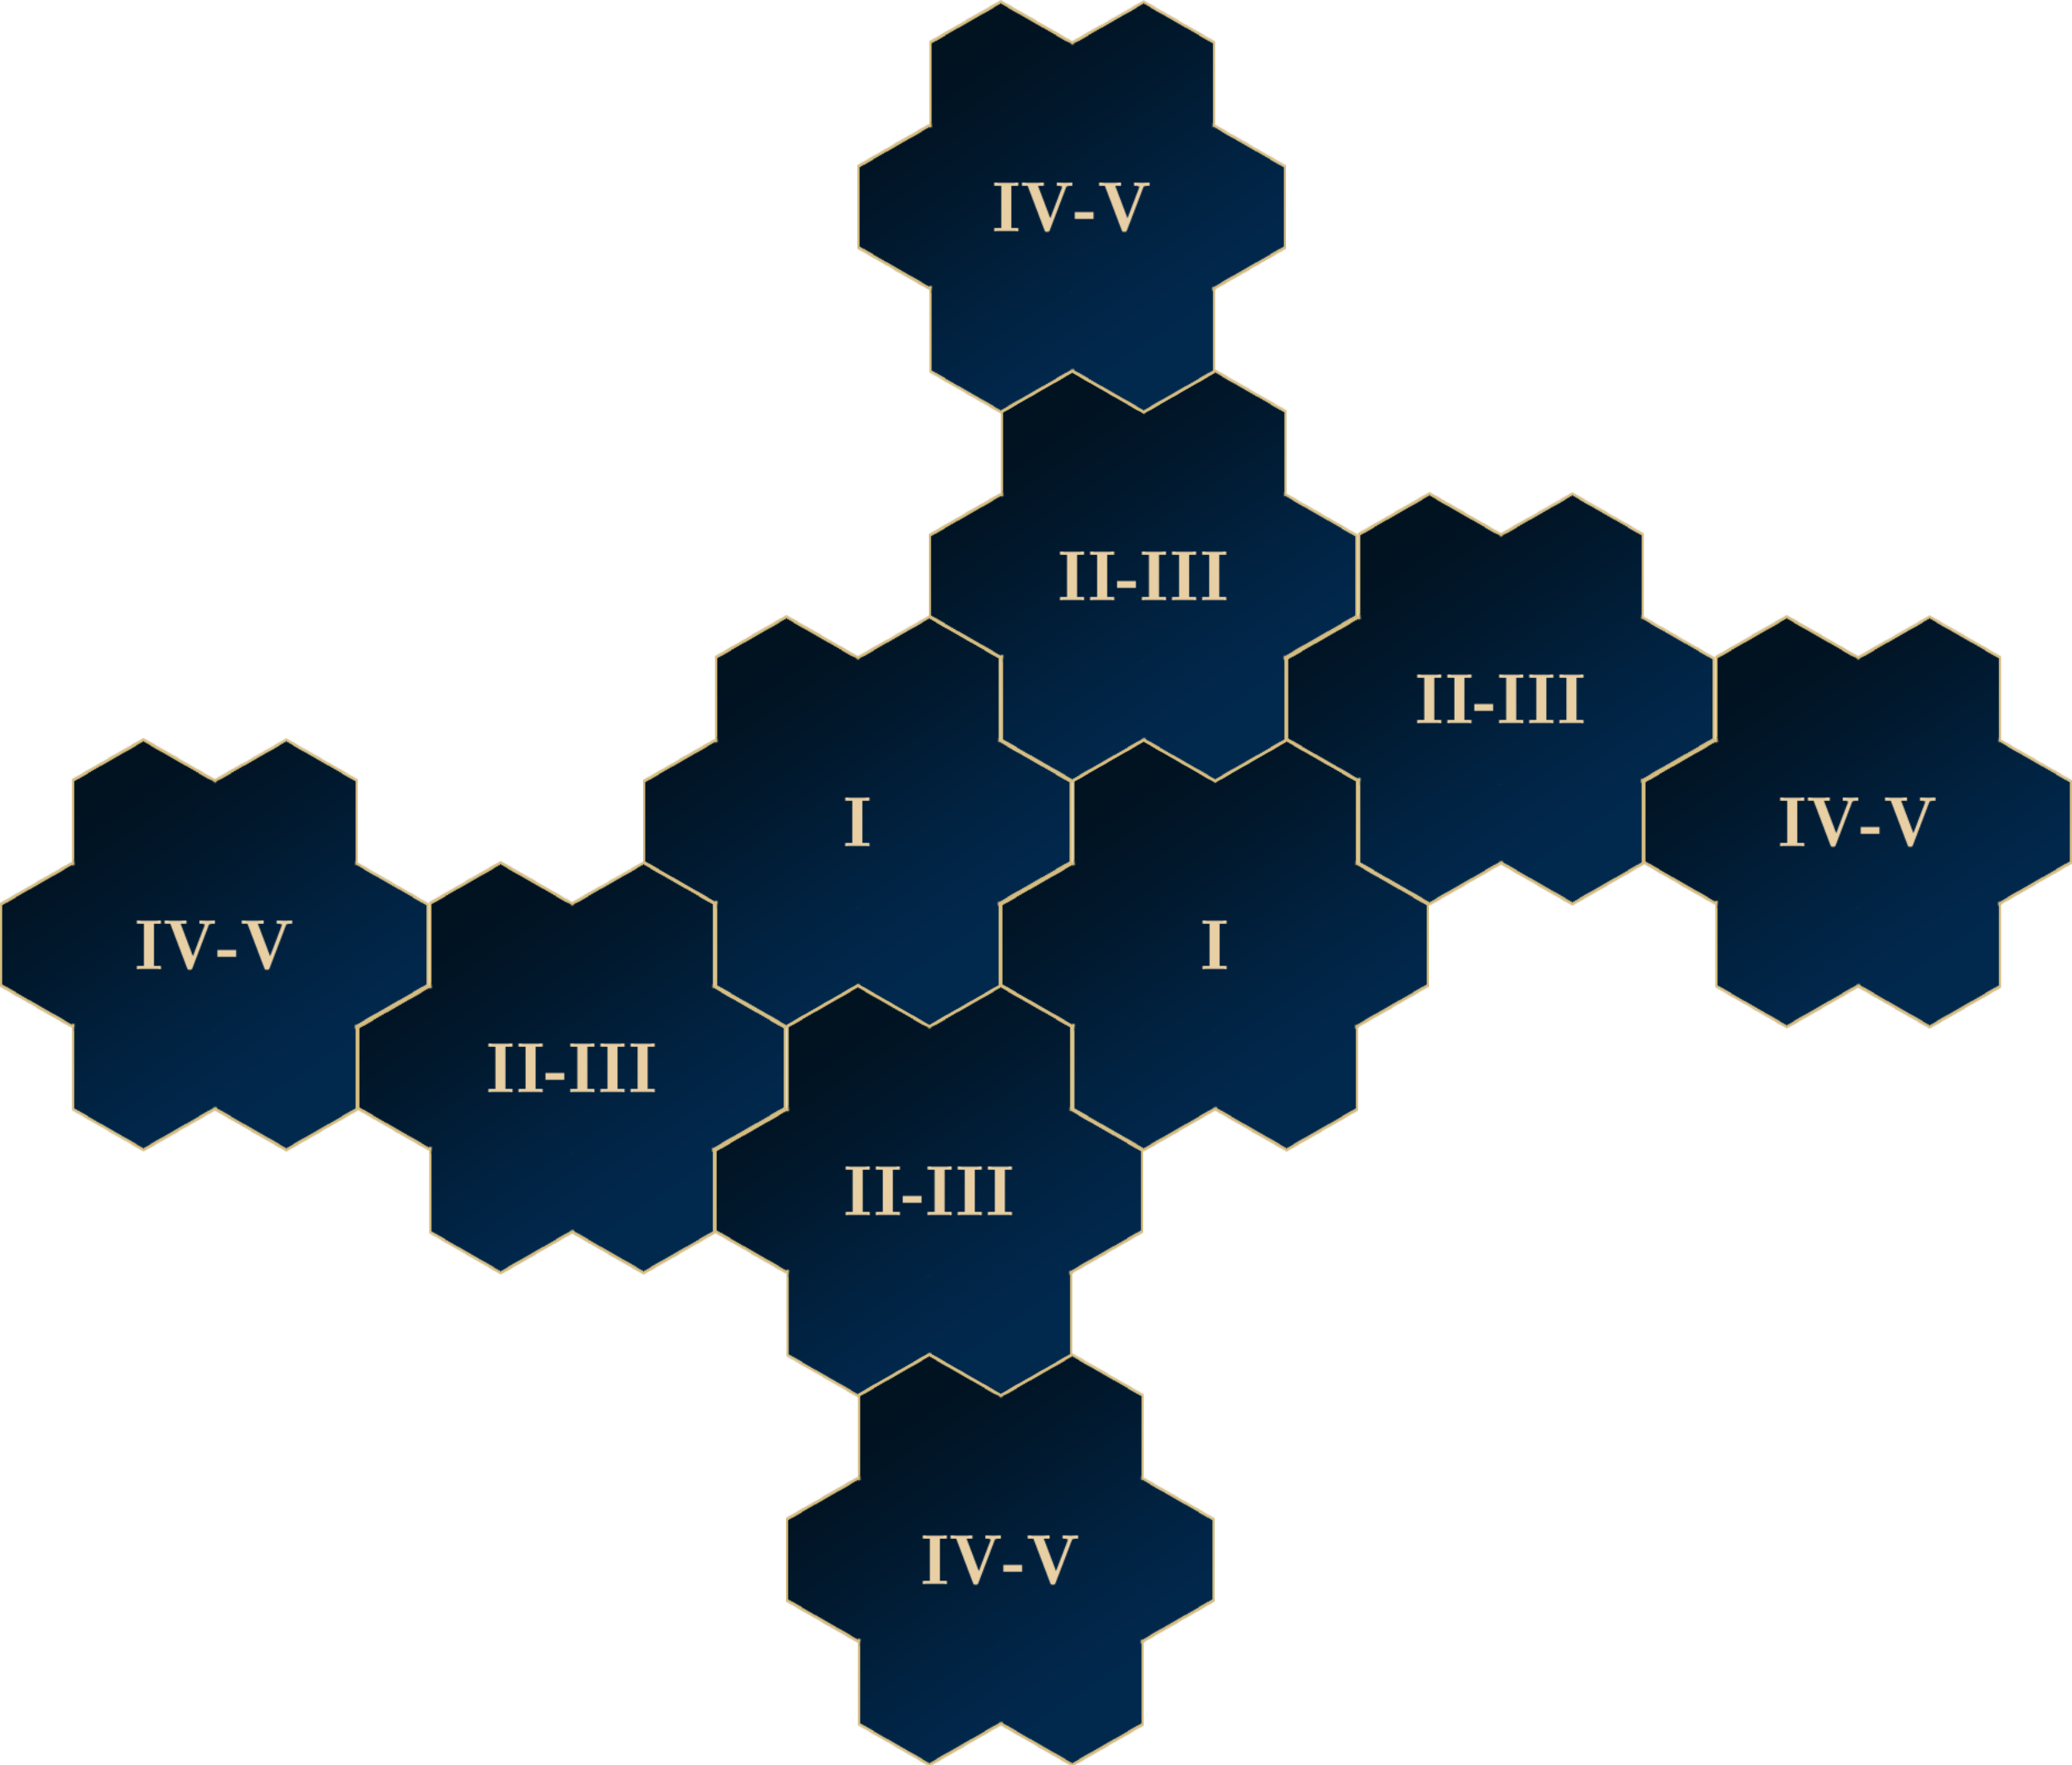
\includegraphics[width=0.6\paperwidth]{\_assets/maps/sentinels.png}

\footnotetext[1]{Always 1 unit of Azure Dragons (starting units of Boss Army). The rest is random\label{azure}.}


\end{document}
